%% 歩容パターンの再評価手法の実装.tex
%% LaTeX-2e 専用

\chapter{歩容パターンの再評価手法の実装}\label{chapter:歩容パターンの再評価手法の実装}
第\ref{chapter:歩容パターンの再評価手法の実装}章では,
第\ref{chapter:歩容パターンの再評価手法の提案}章で述べた歩容パターンの再評価手法の実装方法について述べる.

\section{グラフ探索による自由歩容パターン生成手法の実装}
再評価手法の実装方法の説明の前に,3次元空間におけるグラフ探索による自由歩容パターン生成手法の実装方法について述べる.
波東らが用いた自由歩容パターン生成手法による直進動作と同様の手法によって歩容パターンを生成しているが,
より早い処理の実現やプログラムの可読性・拡張性の向上のため,その実装方法を1部変更している.
加えて,新たに3次元空間における旋回動作の実装と先行研究の手法の統合を行ったため,変更点を含め,改めて実装方法を説明する.

プログラムの実装はC++20を用いて行っており,命名規則はGoogle~C++~Style~Guide\cite{cita:google_cpp_style_guide}にしたがっている.
開発にはVisual~Studio~2022を用いており,プログラムのビルドにはVisual~Studio~2022のMSVCコンパイラを用いている.

また,この章におけるクラスや構造体の図はUML(Unified~Modeling~Language)を用いて表現されており,
上からクラス・構造体の名前,メンバ変数,メンバ関数を表している.
メンバ変数は,アクセス修飾子,変数名,型の順に記述されており,
メンバ関数は,アクセス修飾子,関数名,引数,戻り値の順に記述されている.
アクセス修飾子は記号を用いて表し,+はpublic,protectedは\#,
privateは$-$である.
クラス間の関係は,継承関係は空白の三角形,集約関係は空白の菱形で表している.
集約関係とは,クラスのメンバ変数として他のクラスを持つことを表している.

\subsection{プログラム全体の流れ}
グラフ探索による自由歩容パターン生成手法では,
歩容パターングラフの作成,歩容パターングラフの探索の2つの処理を行う.
歩容パターングラフを作成する処理はGraphTreeCreatorクラスで実装されており,
歩容パターングラフの探索を行う処理はGraphSearcherクラスで実装されている.

これらの処理の流れを\figref{fig:graph_search_sequence}に示す.
まず,GraphTreeCreatorクラスに現在のロボットの状態を表すノードを渡す.
GraphTreeCreatorクラスは渡されたノードを根ノードとする歩容パターングラフを作成する.
次に,GraphSearcherクラスに作成された歩容パターングラフを渡す.
このとき値をコピーして渡すのではなく,
ポインタを渡すことでメモリの使用量を削減するとともに,
グラフ探索の処理時間を短縮している.
GraphSearcherクラスは渡された歩容パターングラフを探索し,
最適な次の動作を見つけて返す.
以上の流れでグラフ探索による自由歩容パターン生成手法を実装している.

\figref{fig:graph_search_class_diagram}にグラフ探索による自由歩容パターン生成手法を実装したクラスのクラス図を示す.
GaitPatternGeneratorBasicクラスは,自由歩容パターン生成手法を実装したクラスである.
GaitPatternGeneratorBasicクラスは,IGaitPatternGeneratorインターフェイスを継承しており,
メンバ関数としてGetNextNodeByGraphSearch関数を持っている.
GetNextNodeByGraphSearch関数は,現在のロボットの状態を表すノードを引数,
地形の情報,目標位置・目標姿勢を引数に取り,グラフ探索によって最適な歩容パターンを返す.
IGaitPatternGeneratorインターフェイスを介することで,
後述する再評価手法の実装や,グラフ探索による自由歩容パターン生成手法の切り替えを容易にしている.
メンバ変数にGraphTreeCreatorクラスのポインタと,
IGraphSearcherインターフェイスを継承したクラスのポインタをもっており,
GaitPatternGeneratorBasicクラスのコンストラクタでそれぞれ初期化される.

GraphTreeCreatorクラスは,歩容パターングラフの作成を行うクラスである.
メンバ変数にINodeCreatorインターフェイスのポインタの配列を持っており,
行う動作によって異なるINodeCreatorクラスを用いてグラフを作成する.
IGraphSearcherインターフェイスは,グラフ探索を行う処理を表すインターフェイスである.
歩容パターングラフの作成,歩容パターングラフの探索はそれぞれ
行う動作によって異なる方法で処理を行うためインターフェイスを作成している.

\begin{figure}[htbp]
  \begin{center}
    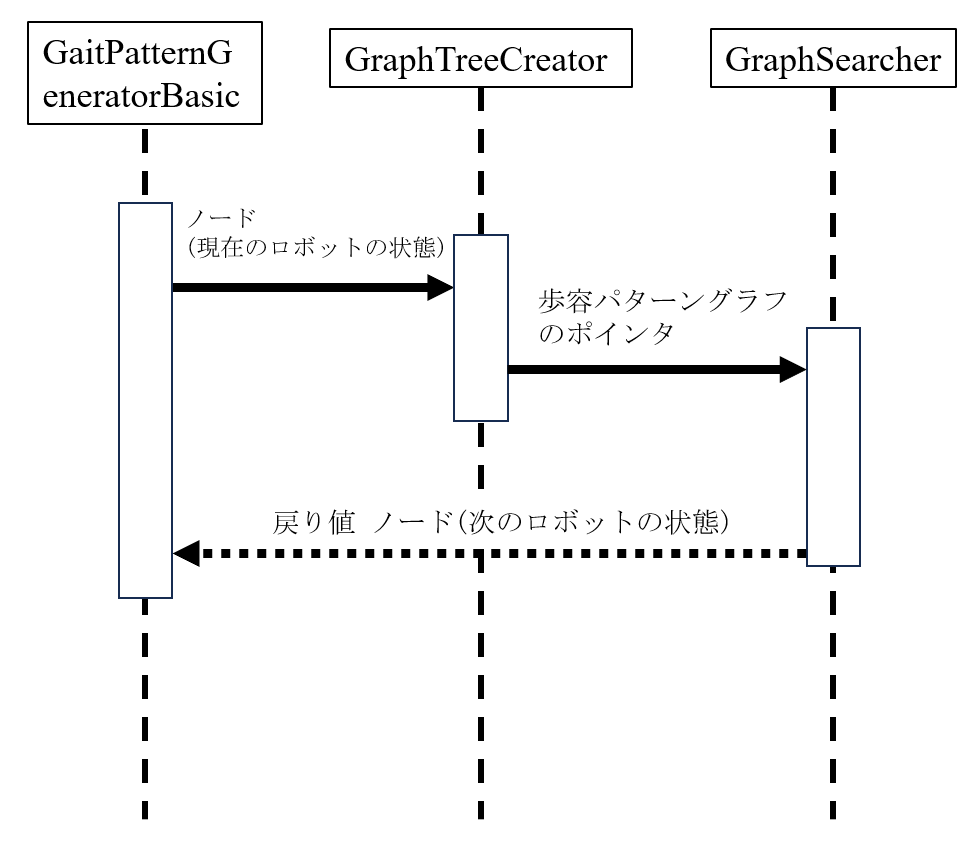
\includegraphics[width=65mm, clip]{figure/chapter3/sequence_main.png}
    \caption{Graph Search Sequence}
    \label{fig:graph_search_sequence} % chktex 24
  \end{center}
\end{figure}

\begin{figure}[htbp]
  \centering
  \begin{tikzpicture}  % [show background grid]
    \begin{interface}[text width=70mm]{IGaitPatternGenerator}{-12, -7.5}
      \attribute{}
      \operation{+ GetNextNodeByGraphSearch() }
    \end{interface}

    \begin{class}[text width=70mm]{GaitPatternGeneratorBasic}{-12, 0}
      \implement {IGaitPatternGenerator}
      \attribute{- graph\_searcher\_ptr\_ : std::unique\_ptr\textless~IGraphSearcher~\textgreater}
      \attribute{- graph\_tree\_creator\_ptr\_ : std::unique\_ptr\textless~GraphTreeCreator~\textgreater}
      \attribute{- graph\_tree\_ : GaitPatternGraphTree}
      \operation{+ GetNextNodeByGraphSearch(\newline
      \qquad current\_node : RobotStateNode, \newline 
      \qquad map : MapState, \newline 
      \qquad operation : RobotOperation, \newline
      \qquad output\_node\_ptr : RobotStateNode*) : \newline
      \qquad void }
    \end{class}

    \begin{interface}[text width=60mm]{IGraphSearcher}{-4, -4}
      \attribute{}
      \operation{+ SearchGraphTree() }
    \end{interface}

    \begin{class}[text width=60mm]{GraphTreeCreator}{-4, 0}
      \attribute{- node\_creator\_map\_ : std::map\textless~HexapodMove, std::unique\_ptr\textless~INodeCreator~\textgreater~\textgreater}
      \operation{+ Init() }
      \operation{+ CreateGraphTree() }
    \end{class}

    \begin{class}[text width=60mm]{GaitPatternGraphTree}{-4, -7}
      \attribute{- nodes\_ : std::vector\textless~RobotStateNode~\textgreater}
      \attribute{- graph\_size\_ : int}
    \end{class}

    \aggregation{GaitPatternGeneratorBasic}{}{}{IGraphSearcher}
    \aggregation{GaitPatternGeneratorBasic}{}{}{GraphTreeCreator}
    \aggregation{GaitPatternGeneratorBasic}{}{}{GaitPatternGraphTree}

  \end{tikzpicture}
  \caption{Graph Search Class Diagram}
  \label{fig:graph_search_class_diagram}  % chktex 24
\end{figure}

\newpage

\subsection{ノードを表現する構造体}
次に,歩容パターングラフを作成する処理を記述するために,ノードについて説明する.
歩容パターングラフのノードは\figref{fig:robot_state_node}のような,
ロボットの状態を表す構造体RobotStateNodeで表現した.
歩容パターングラフではRobotStateNodeを配列とすることで作成するため,
RobotStateNode構造体はサイズを小さくし,メモリの使用量を少なくすることが求められる.

RobotStateNodeのメンバ変数leg\_stateは,ロボットの脚の状態を表すビット列である.
C++の標準ライブラリのstd::bitsetを用いて実装されており,28ビットの長さを持つ.
ビット列の各ビットは,\figref{fig:leg_state_bit}のように定義されている.
下位24bitは各脚の離散化された脚位置と遊脚状態を表し,上位4bitは後述するロボットの重心位置を表す.
このようにすることで複数のパラメータを1つの変数のみで表現することができ,
メモリの使用量を削減することができる.

leg\_posとleg\_reference\_posは,ロボットの脚の位置を表すVector3構造体の配列である.
Vector3構造体は,3次元ベクトルを表す構造体であり,\figref{fig:vector3}のように定義されている.
leg\_posはロボットの脚の現在の位置を表し,leg\_reference\_posは離散化された脚位置の脚位置4の位置を表す.
座標系は脚の付け根を原点とするローカル座標系であり,単位はmmである.

center\_of\_mass\_global\_coordとpostureは,
グローバル座標におけるロボットの重心位置と姿勢を表すVector3構造体とQuaternion構造体である.
Quaternion構造体は,クォータニオンを表す構造体であり,\figref{fig:quaternion}のように定義されている.

next\_moveは,次に行う動作を表すHexapodMove列挙型である.
先行研究ではint型で表現していたが,可読性の向上のために列挙型を用いている.
parent\_indexは,親ノードのインデックスを表すint型である.
先行研究では親ノードへのポインタを用いていたが,
自身の実行環境ではポインタのサイズは8byteであるため,
4byteのint型を用いることでメモリの使用量を削減している.
depthは,ノードの深さを表すint型である.
RobotStateNodeは以上のように定義されており,188byteのサイズである.

このノードを用いて歩容パターングラフを作成する際,
根ノードはparent\_indexを$-1$,depthを$0$に設定する.
その後,根ノードのnext\_moveを基に子ノードを作成し,
parent\_indexを根ノードのインデックス,depthを$1$に設定する.
こうして作成した子ノードのnext\_moveを基に,
さらに子ノードを作成することで歩容パターングラフを作成できる.
歩容パターングラフはRobotStateNode構造体の配列で表現できるが,
処理を簡単にするためGaitPatternGraphTreeクラスでラッパーしている.

RobotStateNode構造体とVector3構造体,Quaternion構造体は
それぞれメンバ変数を操作するためのメンバ関数を持っているが,
グラフ探索の処理とは直接的な関係がないため,ここでは説明を省略する.
\\ 

\begin{figure}[htbp]
  \centering
  \begin{tikzpicture}
    \begin{class}[text width=8cm]{RobotStateNode}{0, 0}
      \attribute{+ leg\_state : std::bitset\textless 28\textgreater}
      \attribute{+ leg\_pos : std::array\textless Vector3, 6\textgreater}
      \attribute{+ leg\_reference\_pos : std::array\textless Vector3, 6\textgreater}
      \attribute{+ center\_of\_mass\_global\_coord : Vector3}
      \attribute{+ posture : Quaternion}
      \attribute{+ next\_move : HexapodMove}
      \attribute{+ parent\_index : int}
      \attribute{+ depth : int} 
      \operation{}
    \end{class}
  \end{tikzpicture}
  \caption{RobotStateNode Struct}
  \label{fig:robot_state_node}  % chktex 24
\end{figure}

\begin{figure}[htbp]
  \begin{tabular}{cc}
    \begin{minipage}[t]{0.45\hsize}
      \centering
      \begin{tikzpicture}
        \begin{class}[text width=6cm]{Vector3}{0, 0}
        \attribute{+ x : float}
        \attribute{+ y : float}
        \attribute{+ z : float}
        \operation{}
        \end{class}
      \end{tikzpicture}
      \caption{Vector3 Struct}
      \label{fig:vector3}  % chktex 24
    \end{minipage}
    &
    \begin{minipage}[t]{0.45\hsize}
      \centering
      \begin{tikzpicture}
        \begin{class}[text width=6cm]{Quaternion}{0, 0}
          \attribute{+ w : float}
          \attribute{+ v : Vector3}
          \operation{}
        \end{class}
      \end{tikzpicture}
      \caption{Quaternion Struct}
      \label{fig:quaternion}  % chktex 24
    \end{minipage}       
  \end{tabular}
\end{figure}

\begin{figure}[htbp]
  \begin{center}
    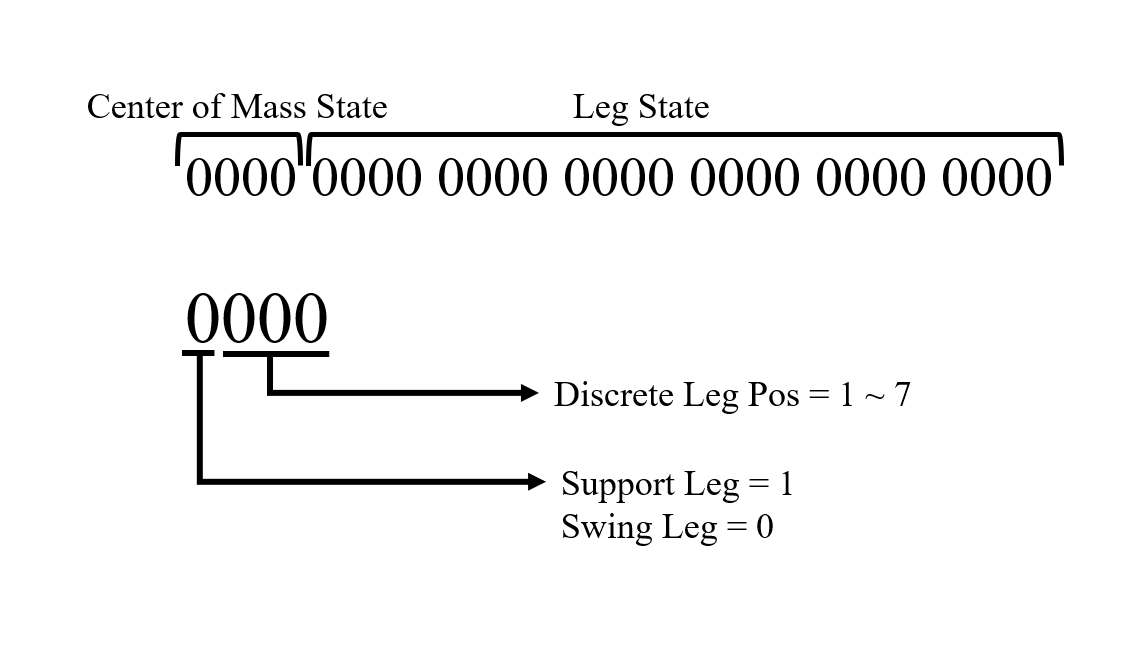
\includegraphics[width=80mm, clip]{figure/chapter3/leg_state.png}
    \caption{Leg State Bit}
    \label{fig:leg_state_bit} % chktex 24
  \end{center}
\end{figure}

\subsection{目標位置・目標姿勢を表現する構造体}
ロボットの目標位置・目標姿勢を表現するRobotOperation構造体を\figref{fig:robot_operation}に示す.
メンバ変数のoperation\_type\_はロボットの動作を表す列挙型,RobotOperationType型の変数である.
この変数の値によってロボットの行うべき動作が決定される.
これはつまり,グラフ探索において高く評価されるノードが変更されるということである.
operation\_type\_以外の変数は具体的にどのような動作を行うかを表し,
operation\_type\_の値によって使用する変数が決定される.

operation\_type\_の値と使用する変数の対応を\tableref{tab:robot_operation_type_enum}に示す.
直進動作を行う場合,指定することができるのはkStraightMoveVectorとkStraightMovePositionの2つである.
kStraightMoveVectorは,ロボットの進行方向を単位ベクトルのstraight\_move\_vector\_で指定する.
kStraightMovePositionは,ロボットの目標位置をstraight\_move\_position\_で指定する.

その場旋回動作を行う場合,指定することができるのはkSpotTurnLastPostureとkSpotTurnRotAxisの2つである.
kSpotTurnLastPostureは,ロボットの旋回前の姿勢をspot\_turn\_last\_posture\_で指定する.
kSpotTurnRotAxisは,ロボットの旋回軸をspot\_turn\_rot\_axis\_で指定し,その軸周りに右ねじの方向に旋回する.
\\

% RobotOperation 構造体の説明
\begin{figure}[h]
  \centering
  \begin{tikzpicture}
    \begin{class}[text width=7cm]{RobotOperation}{0, 0}
      \attribute{+ operation\_type\_ : RobotOperationType}
      \attribute{+ straight\_move\_vector\_ : Vector3}
      \attribute{+ straight\_move\_position\_ : Vector3}
      \attribute{+ spot\_turn\_last\_posture\_ : Quaternion}
      \attribute{+ spot\_turn\_rot\_axis\_ : Vector3}
      \operation{}
    \end{class}
  \end{tikzpicture} 
  \caption{RobotOperation Struct}
  \label{fig:robot_operation}  % chktex 24
\end{figure}

% RobotOperationTypeの列挙型をテーブルにする
\begin{table}[h]
  \caption{RobotOperationType Enum}
  \label{tab:robot_operation_type_enum}  % chktex 24
  \begin{center}
    \begin{tabular}{|c|c|} \hline  % chktex 44
      \backslashbox{動作}{要素} & RobotOperationType \\ \hline  % chktex 44
      \multirow{2}{*}{直進} & kStraightMoveVector \\ \cline{2-2}  % chktex 44
      & kStraightMovePosition \\ \hline  % chktex 44
      \multirow{2}{*}{その場旋回} & kSpotTurnLastPosture \\ \cline{2-2}  % chktex 44
      & kSpotTurnRotAxis \\ \hline  % chktex 44
    \end{tabular}
  \end{center}
\end{table}

\newpage

\subsection{地形を表現する構造体}
地形を表現するMapState構造体を\figref{fig:map_class_diagram}に示す.
グラフ探索においては連続的な地形を離散化する必要があるため,
地形を離散化するための点群を表す配列map\_point\_をメンバ変数に持っている.
map\_point\_はVector3構造体の配列であり,脚の接地可能点を表す.
map\_point\_は地形を上から見た時,格子状に配置されており,
隣の脚接地可能点との間隔は一定で$20 [mm]$である.
この間隔はロボットの脚先の面積を考慮して決定した.

MapState構造体を用いることで地形を離散化することができるが,
依然として脚接地可能点の数は多い.
そのため,ロボットを中心に地形を分割し,
各分割領域における脚接地可能点を表すDividedMapState構造体を作成した.
\figref{fig:map_view}において,赤い点で表される脚接地可能点がDividedMapState構造体で表現されている.
DividedMapState構造体は,グローバル座標におけるロボットの重心位置を表すglobal\_robot\_com\_を中心に
地形を分割した際の,各分割領域における脚接地可能点を表すdivided\_map\_point\_をメンバ変数に持っている.
また,各分割領域の最上点の高さを表すdivided\_map\_top\_z\_をメンバ変数に持っている.
脚の接地判定を行う際は,DividedMapState構造体の中から脚先に近い領域群を選択し,
その領域群における脚接地可能点を用いて接地判定を行うことで,
計算する脚接地可能点の数を減らしている.
\\

% MapState 構造体の説明
\begin{figure}[h]
  \centering
  \begin{tikzpicture}
    \begin{class}[text width=7cm]{MapState}{0, 2}
      \attribute{+ map\_point\_ : std::vector~\textless~Vector3~\textgreater}
      \operation{}
    \end{class}

    \begin{class}[text width=7cm]{DividedMapState}{0, 0}
      \attribute{+ global\_robot\_com\_ : Vector3}
      \attribute{+ divided\_map\_point\_ : std::vector~\textless~std::vector~\textless~Vector3~\textgreater~\textgreater}
      \attribute{+ divided\_map\_top\_z\_ : std::vector~\textless~float~\textgreater}
      \operation{}
    \end{class}
  \end{tikzpicture} 
  \caption{MapState Struct}
  \label{fig:map_class_diagram}  % chktex 24
\end{figure}

\begin{figure}[h]
  \begin{center}
    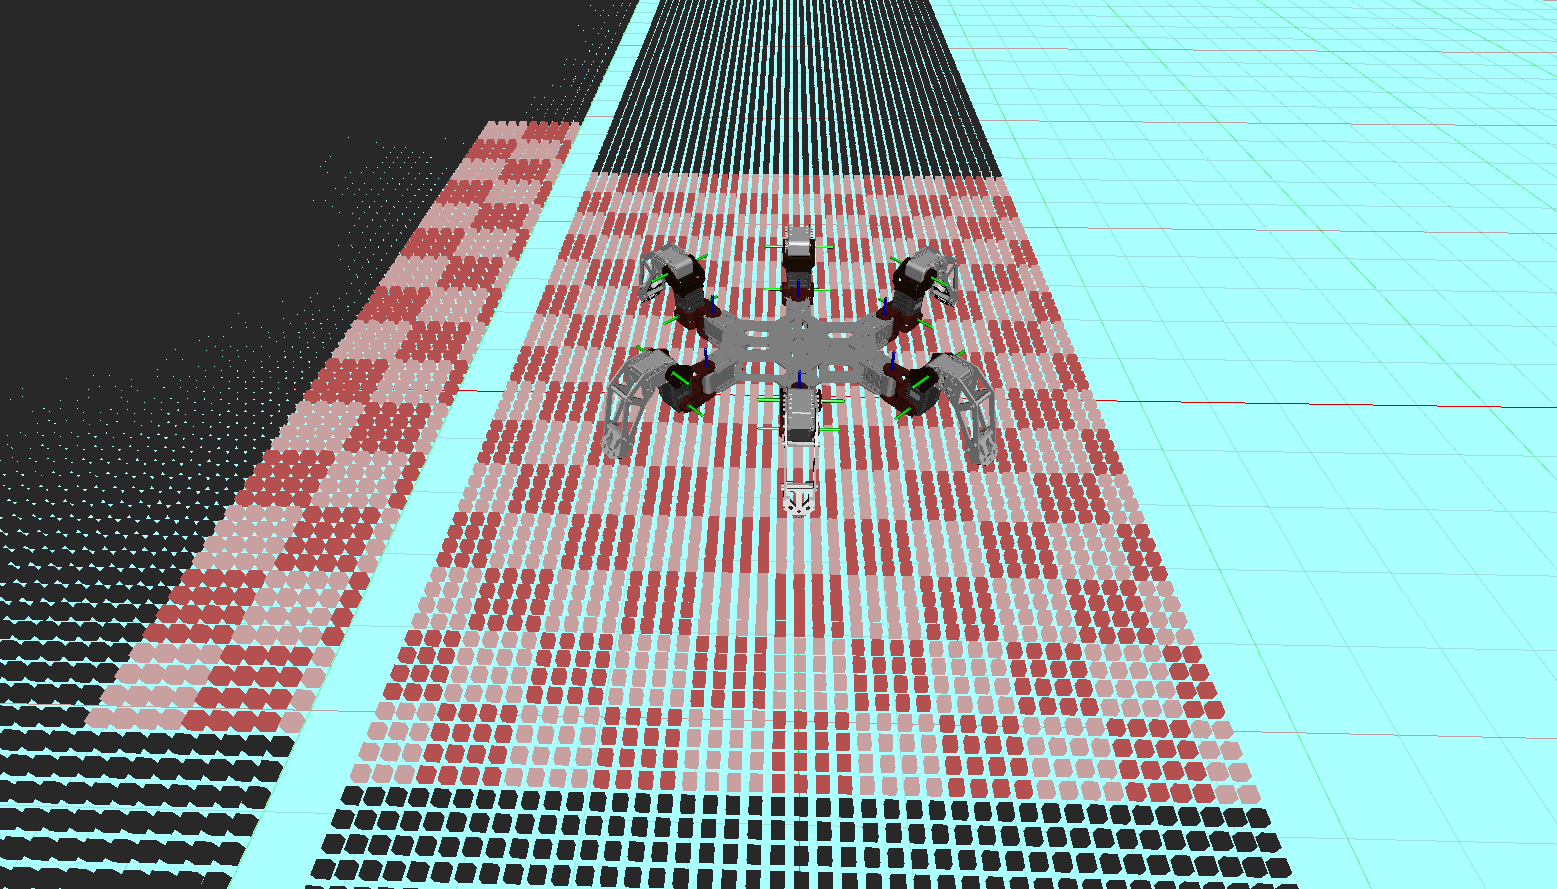
\includegraphics[width=80mm, clip]{figure/chapter3/map_view.png}
    \caption{Map View}
    \label{fig:map_view}  % chktex 24
  \end{center}
\end{figure}


\subsection{子ノードを作成するプログラム}
歩容パターングラフを作成するためには,子ノードを作成するプログラムが必要であり,
そのプログラムをINodeCreatorインターフェイスを実装した各クラスで実装している.
INodeCreatorインターフェイスは\figref{fig:node_creator_class_diagram}のように定義されている.
Create関数は,引数に現在のノード,現在のノードのインデックス,作成した子ノードを格納する配列へのポインタを持っている.
戻り値で結果を返す場合,RobotStateNode構造体のコピー処理が発生するため,
引数で渡した配列のポインタを通じて値を返している.
各クラスでは,Create関数をオーバーライドすることで,子ノードを作成する処理を実装している.

歩容パターングラフの規模を小さくするためには1つの親ノードがもつ子ノードの数は少なくする必要がある.
しかし,数を少なくしすぎると,グラフ探索によって必要な歩容パターンが消えてしまう可能性がある.
各クラスでは1つの親ノードから10個程度の子ノードを作成するようにしており,
深さ5の歩容パターングラフのノード数はが$10^5 \sim 10^6$程度となるようにしている.
ロボットの動作に応じて異なるクラスを用いたため,以下に各クラスの説明を記述する.
\\

% INodeCreator 構造体の説明
\begin{figure}[h]
  \centering
  \begin{tikzpicture}
    \begin{interface}[text width=7cm]{INodeCreator}{0, 0}
      \attribute{}
      \operation{+ Create(current\_node : RobotStateNode, current\_node\_index : int, 
                 output\_graph : std::vector~\textless~RobotStateNode~\textgreater~*) : void }
    \end{interface}
  \end{tikzpicture} 
  \caption{NodeCreator Interface}
  \label{fig:node_creator_class_diagram}  % chktex 24
\end{figure}

\subsubsection{重心の上下移動}
重心の上下移動を行うための処理はNodeCreatorComUpDownクラスで実装している.
NodeCreatorComUpDownクラスは処理を行うノードから,
重心を上下移動させることで作成できる子ノードを戻り値として返す.

重心の移動後の座標は無数に存在するため,\figref{fig:com_up_down}に離散化の様子を示した.
まず,現在の脚位置から下げることが可能な最低の重心高さと,
現在の脚位置から上げることが可能な最大の重心高さを計算する.
この時,近似された脚の可動範囲から脚先が届くかを判定しており,
またDevidedMapStateのdivided\_map\_top\_z\_を用いて,
地形との干渉を考慮している.
次に,最低の重心高さから最大の重心高さまで等間隔で5分割し,
各重心高さにおける子ノードを作成する.
重心の高さを変更しない場合を考慮して,そのままの重心高さを持つ子ノードも作成する.
離散化時の分割数はグラフの規模を考慮して決定した.

\begin{figure}[h]
  \begin{center}
    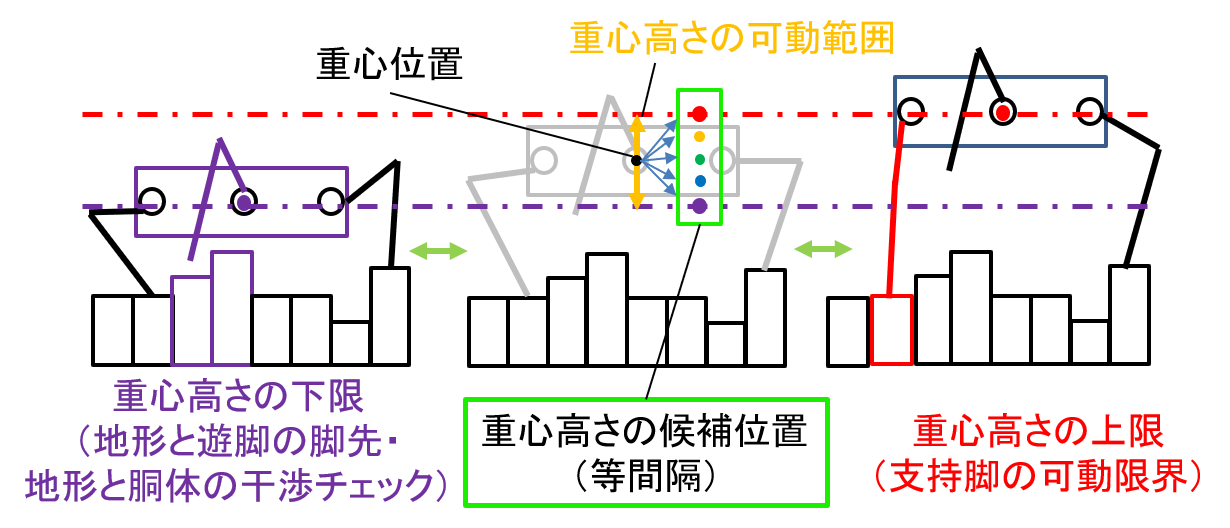
\includegraphics[width=70mm, clip]{figure/chapter3/com_up_down.png}
    \caption{Discretization of  \newline the Vertical Shift of the Center of Mass}
    \label{fig:com_up_down}  % chktex 24
  \end{center}
\end{figure}

\subsubsection{重心の平行移動}
重心の平行移動を行うための処理はNodeCreatorComMoveクラスで実装している.
NodeCreatorComMoveクラスは処理を行うノードから,
重心を平行移動させることで作成できる子ノードを戻り値として返す.

上下移動の場合と同様に,重心の移動後の座標は無数に存在するため以下の手順で離散化を行う.
まず重心を平行移動させる候補領域を\figref{fig:candidate_area_com}のように決定する.
脚先を投影してできる六角形の対角線をすべて結び,その交点から7通りの重心の候補領域を決定する.
そして,それぞれ右前方にあるものから順に1$\sim$6と番号を振る.
また,中央にあるもののうち,ロボットの前方を上としたときに逆三角形となるものを7,
ロボットの後方を上としたときに逆三角形となるものを8とする.

次にこれらの候補領域から実際に重心を平行移動させる地点を決定する.
\figref{fig:determination_of_com}に示すように,候補領域を格子状に分割する.
そして,各格子点において重心を平行移動させた時,
もっとも進行方向への移動量が大きくなる点を選択し子ノードの重心座標とする.
この時に静的安定余裕を確認し,規定された値を下回る場合はその点を選択しない.
また,このときRobotStateNode構造体のleg\_state\_の上位4bitに,
候補領域の番号を離散化された重心位置として格納する.
加えて,RobotStateNode構造体のleg\_reference\_pos\_を現在のleg\_pos\_の値に更新する.

\begin{figure}[h]
  \begin{tabular}{cc}
      \begin{minipage}{0.5\textwidth}
          \centering
          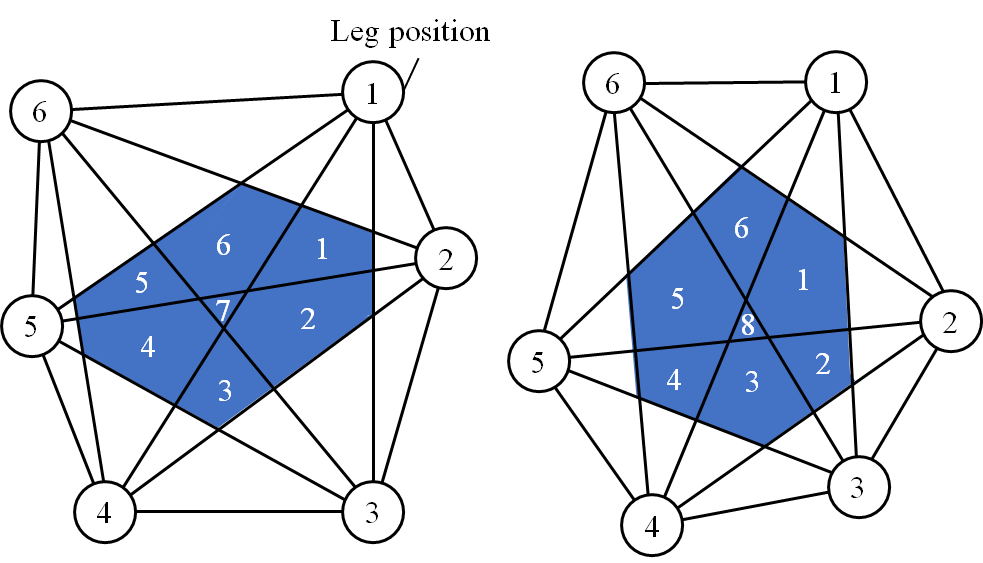
\includegraphics[width=1.0\linewidth]{figure/chapter3/leg_pos_com.png}
          \caption{Candidate Area of Center of Mass}
          \label{fig:candidate_area_com} % chktex 24
      \end{minipage}
      \begin{minipage}{0.5\textwidth}
          \centering
          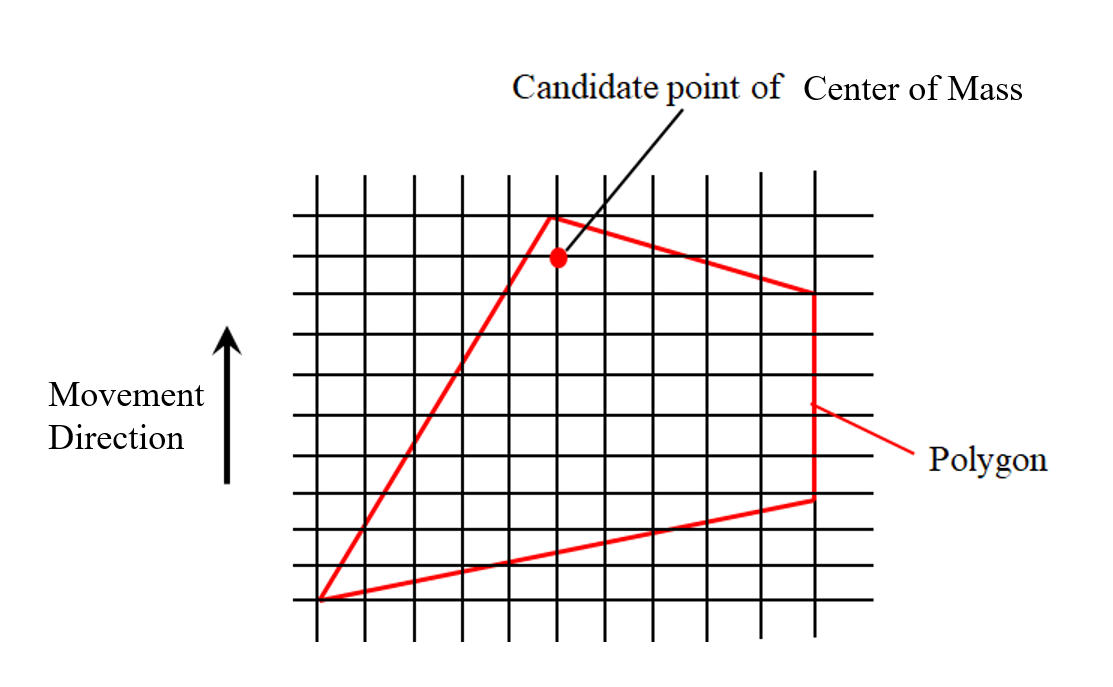
\includegraphics[width=1.0\linewidth]{figure/chapter3/center_of_mass.png}
          \caption{Determination of Center of Mass}
          \label{fig:determination_of_com} % chktex 24
      \end{minipage}
  \end{tabular}
\end{figure}

\subsubsection{胴体の回転移動}
胴体の回転運動を行うための処理はNodeCreatorBodyRotクラスで実装している.
NodeCreatorBodyRotクラスは処理を行うノードから,
胴体を回転させることで作成できる子ノードを戻り値として返す.

重心を中心として,重力の方向を軸とした回転運動を行う.
回転量は$-20 \sim 20 [\deg]$の範囲を$2 [\deg]$刻みで離散化しており,
1つのノードにつき21個の子ノードを作成する.
回転運動を行う際には,近似された脚の可動範囲から脚先が届くかを判定しており,
届かない場合,そのノードは作成しない.

\subsubsection{脚の上下運動・水平運動}
\chref{chapter:歩容パターンの再評価手法の提案}で述べたように,
脚の水平運動は脚の状態が等しく,別の階層にあるノード間での遷移で行うことができ,
脚の上下運動は同じ階層にあるノード間での遷移で行うことができる.
脚の状態が等しく,別の階層にある子ノードを生成する処理はNodeCreatorLegHierarchyクラスで実装しており,
同じ階層にある子ノードを生成する処理はNodeCreatorLegUpDownクラスで実装しているため,
まずは,NodeCreatorLegHierarchyクラスの説明を行う.

NodeCreatorLegHierarchyクラスでは,処理を行うノードの脚の状態を表すleg\_state\_から,
遊脚している脚を取得し,その脚の離散化された脚位置を$1 \sim 7$に変更した子ノードを作成する.
つまり1脚遊脚している場合は7つの子ノードを作成し,
3脚遊脚している場合は$7^3 = 343$の子ノードを作成する.
このクラスでは実際の脚位置を変更するのではなく,あくまで脚の状態を表すleg\_state\_を変更するのみである.

次にNodeCreatorLegUpDownクラスを説明する.
NodeCreatorLegUpDownクラスでは,処理を行うノードの脚の状態を表すleg\_state\_から,
遊脚の組み合わせを変更した子ノードを作成する.
遊脚の組み合わせのうち,接地しえない脚がある組み合わせは作成しないようにするため,
最初に現在遊脚中の各脚について,その脚が離散化された脚位置で指定された脚位置に接地することができるかを判定する.
また,重心の位置から静的安定性を保つことができない場合も作成しない.
処理の流れを以下に示す.

\begin{enumerate}
  \item 離散化された重心位置から同時に遊脚することができない隣り合う2脚を遊脚するノードを削除する\par
        RobotStateNodeのleg\_state\_から重心位置を取得し,
        その重心位置から同時に遊脚することができない隣り合う2つの脚を,
        同時に遊脚するノードを作成する候補から削除する.
        \tableref{tab:leg_combination_table}にある重心位置において,同時に遊脚することができない脚の組み合わせを示す.
        この表における重心位置や脚の番号は\figref{fig:candidate_area_com}のものと同じである.
  \item 離散化された脚位置で指定された位置に接地可能な点があるか確認する\par
        各脚ごとにRobotStateNodeのleg\_state\_から離散化された脚位置を取得し,
        その脚位置で指定された脚位置に接地可能な点があるかを確認する.
        接地可能な点がない場合,その脚を接地するノードを作成する候補から削除する.
        接地可能な点が複数ある場合はもっとも移動方向への移動量が大きくなる点を選択する.
  \item 子ノードを作成する\par
        (1)(2)の処理の中で候補から削除されなかった,階層内のノードを作成し,これらを子ノードとして返す.
\end{enumerate}

% 連続する2脚のうち,同時に遊脚することができない脚の組み合わせのテーブル
\begin{table}[h]
  \caption{Leg Combination Table}
  \label{tab:leg_combination_table}  % chktex 24
  \begin{center}
    \begin{tabular}{|c|c|c|} \hline  % chktex 44
      重心位置 & 遊脚可能な組 & 遊脚不可能な組  \\ \hline  % chktex 44
      1 & (3,4) (4,5) (5,6) & (6,1) (1,2) (2,3) \\ \hline  % chktex 44
      2 & (4,5) (5,6) (6,1) & (1,2) (2,3) (3,4) \\ \hline  % chktex 44
      3 & (5,6) (6,1) (1,2) & (2,3) (3,4) (4,5) \\ \hline  % chktex 44
      4 & (6,1) (1,2) (2,3) & (3,4) (4,5) (5,6) \\ \hline  % chktex 44
      5 & (1,2) (2,3) (3,4) & (4,5) (5,6) (6,1) \\ \hline  % chktex 44
      6 & (2,3) (3,4) (4,5) & (5,6) (6,1) (1,2) \\ \hline  % chktex 44
      7 & (2,3) (4,5) (6,1) & (1,2) (3,4) (5,6) \\ \hline  % chktex 44
      8 & (1,2) (3,4) (5,6) & (2,3) (4,5) (6,1) \\ \hline  % chktex 44
    \end{tabular}
  \end{center}
\end{table}

\subsubsection{直進動作時におけるノード生成の順番}
直進動作を行う時の,未探索のノードから遷移可能なノードをグラフに追加する際のルールについて説明する.
RobotStateNodeのnext\_move\_には,次の動作を表すHexapodMove型の変数が格納されている.
この変数の値によってどのNodeCreatorクラスを使用するかが決定される.
それぞれのNodeCreatorクラスは子ノードを作成する際に,
親ノードのnext\_move\_の値から子ノードのnext\_move\_の値を以下のルールに基づいて決定する.

\begin{itemize}
  \item 親ノード:脚の水平運動 → 子ノード:脚の上下運動
  \item 親ノード:脚の上下運動 → 子ノード:重心の上下移動
  \item 親ノード:重心の上下移動 → 子ノード:重心の平行移動
  \item 親ノード:重心の平行移動 → 子ノード:脚の水平運動
\end{itemize}

\noindent また,使用するNodeCreatorクラスは以下の4つである.

\begin{itemize}
  \item NodeCreatorLegUpDown
  \item NodeCreatorComUpDown
  \item NodeCreatorComMove
  \item NodeCreatorLegHierarchy
\end{itemize}

このようなルールを定めることによって明らかに無意味な動作
(たとえば,重心を上げる→重心を下げる動作を繰り返すものなど)
を生成することをあらかじめ防ぐことができる.
なお,直進動作以外の動作を行う場合は別のルールを用いてグラフを作成している.

\subsection{グラフ探索時のノードの評価方法}
グラフ探索時では歩容パターングラフのもっとも深いノードをすべて比較し,
最高評価となったノードへのパスから深さ1のノード次のノードとして返す.
RobotOperationで与えられた動作に対して,適切な動作を行うRobotStateNodeを評価するために,
グラフ探索時には複数のノードの評価項目がある.
IGraphSearcherを継承した具象クラスではノードを評価する関数を複数持っており,
それぞれの関数で評価項目を計算している.
この章では3次元空間の直進動作におけるノードの評価方法を説明する.

3次元空間の直進動作のグラフ探索はGraphSearcherStraightMoveクラスで実装している.
処理の流れを以下に示す.

\begin{enumerate}
  \item 高さの評価\par
        進行方向の地形の最大高さを確認し,その地点を歩行するために必要な最低の重心高さを求める.
        求めた重心高さと現在の重心高さの差を評価値として使用し,値が小さいほど評価を高くする,
        現在の最高評価ノードと比較して評価が高ければ最高評価ノードを更新する.
  \item 移動量の評価\par
        (1)が最大評価ノードと同じであれば,直進動作の移動量を評価する.
        まず,根ノードから評価を行うノードまでの移動量を計算する.
        目標方向と移動量の内積を計算し,その値が大きいほど評価を高くする.
        RobotOperationで目標位置が指定されている場合は,
        根ノードから目標位置までの移動ベクトルを正規化したものを目標方向として使用する.
        現在の最高評価ノードと比較して評価が高ければ最高評価ノードを更新する.        
  \item 脚の回転角度の平均値の評価\par
        (2)も最大評価ノードと同じであれば,脚の回転角度の平均値を評価する.
        根ノードと評価を行うノードの脚の回転角度の平均値を計算し,
        その値が大きいほど評価を高くする.
        現在の最高評価ノードと比較して評価が高ければ最高評価ノードを更新する.
\end{enumerate}

\section{歩容パターンの再評価手法の実装}
歩容パターンの再評価手法はIGaitPatternGeneratorインターフェイスを継承したクラスを作成することで実装できる.
IGaitPatternGeneratorインターフェイスを用いたことで,
デコレーターパターンを用いて容易に再評価手法を実装している.
デコレーターパターンとは,既存のクラスに新たな機能を追加するためのデザインパターンである.
デコレータ(デコレータパターンを用いて作られたクラス)はあるインターフェイスを継承するかつ,
自身と同じインターフェイスを継承したクラスをメンバ変数として持つ.
そしてメンバ関数を呼び出す際に,メンバ変数のメンバ関数と自身の持つ処理を実行することで,
既存のクラスをそのままに新たな機能を追加することができる.

再評価手法はGaitPatternGeneratorRevaluationクラスで実装されている.
GaitPatternGeneratorRevaluationクラスはIGaitPatternGeneratorインターフェイスを継承しており,
メンバ変数にIGaitPatternGeneratorインターフェイスのポインタを2つ持っている.
これらのポインタはコンストラクタで初期化され,
1つ目のポインタは再評価手法を適用する前の歩容パターン生成手法を,
2つ目のポインタは再評価手法を適用した後の歩容パターン生成手法を指している.

メンバ関数であるGetNextNodeByGraphSearch関数が呼ばれた場合,
まず,1つ目のポインタのGetNextNodeByGraphSearch関数を呼び出し結果を取得する.
取得したノードから脚軌道生成を行い,成功した場合はそのノードを返す.
失敗した場合は,2つ目のポインタのGetNextNodeByGraphSearch関数を呼び出し結果を取得する.
こうすることで,\chref{chapter:歩容パターンの再評価手法の提案}で提案した,
脚軌道生成に失敗した場合のみグラフ探索をやり直す処理を実装できる.

再評価時には脚軌道生成の失敗を防ぐために,近似された脚の可動範囲を狭める.
近似された脚の可動範囲は\chref{chapter:歩容パターンの再評価手法の提案}で述べたように,
最小半径を$140 [mm]$に設定すればよいため,
狭めた前と後の脚の可動範囲は以下のような条件に設定する.
また,それぞれを図示したものを\figref{fig:leg_range_revaluation_before}と
\figref{fig:leg_range_revaluation_after}に示す.

\begin{enumerate}
  \item 再評価前\par
        \begin{itemize}
          \item 最小半径を$130 [mm]$に設定
          \item 最大半径は\chref{chapter:歩容パターンの再評価手法の提案}で述べた計算方法で設定
          \item 遊脚高さは$-20 [mm]$に設定
        \end{itemize}
  \item 再評価後\par
        \begin{itemize}
          \item 最小半径を$140 [mm]$に設定
          \item 最大半径は\chref{chapter:歩容パターンの再評価手法の提案}で述べた計算方法で設定
          \item 遊脚高さは$-20 [mm]$に設定
        \end{itemize}
\end{enumerate}

\begin{figure}[htbp]
  \centering
  \begin{tikzpicture}  % [show background grid]
    \begin{interface}[text width=70mm]{IGaitPatternGenerator}{-9, -7}
      \attribute{}
      \operation{}
    \end{interface}

    \begin{class}[text width=70mm]{GaitPatternGeneratorRevaluation}{-12, -2}
      \inherit{IGaitPatternGenerator}
      \attribute{- gait\_pattern\_generator\_ptr\_ : std::unique\_ptr\textless~IGaitPatternGenerator~\textgreater}
      \attribute{- gait\_pattern\_generator\_revaluation\_ptr\_ : std::unique\_ptr\textless~IGaitPatternGenerator~\textgreater}
      \operation{}
    \end{class}

    \begin{class}[text width=50mm]{GaitPatternGeneratorBasic}{-5.5, -4}
      \inherit{IGaitPatternGenerator}
      \attribute{}
      \operation{}
    \end{class}

  \end{tikzpicture}
  \caption{Gait Pattern Generator Revaluation Class Diagram}
  \label{fig:gait_pattern_generator_revaluation}  % chktex 24
\end{figure}

\begin{figure}[h]
  \begin{tabular}{cc}
      \begin{minipage}{0.5\textwidth}
          \centering
          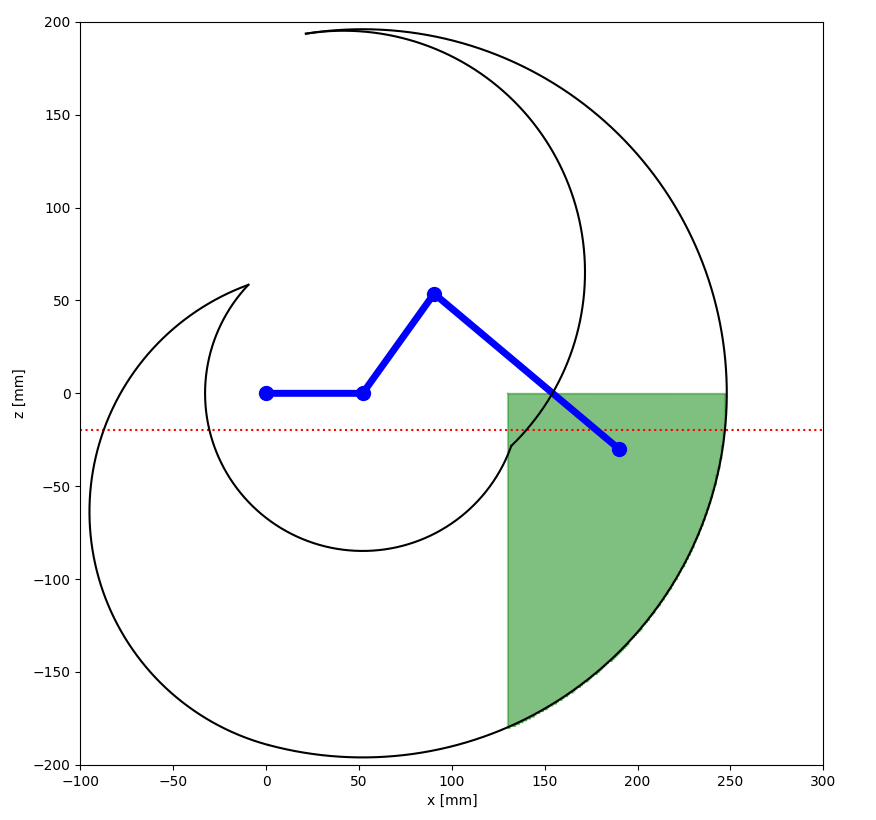
\includegraphics[width=1.0\linewidth]{figure/chapter3/revaluetion_before.png}
          \caption{Leg Range Before Revaluation}
          \label{fig:leg_range_revaluation_before} % chktex 24
      \end{minipage}
      \begin{minipage}{0.5\textwidth}
          \centering
          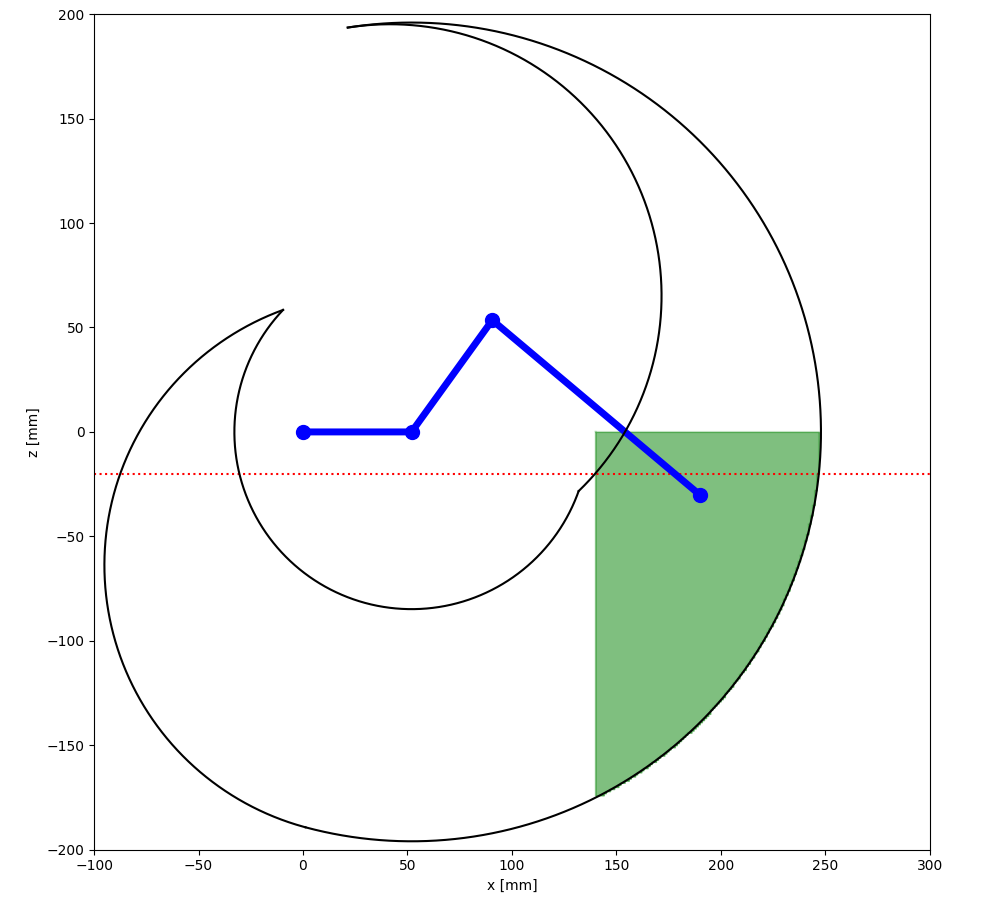
\includegraphics[width=1.0\linewidth]{figure/chapter3/revaluetion_after.png}
          \caption{Leg Range After Revaluation}
          \label{fig:leg_range_revaluation_after} % chktex 24
      \end{minipage}
  \end{tabular}
\end{figure}

\newpage

\section{グラフ探索による自由歩容パターン生成手法の統合}
先行研究において,グラフ探索による自由歩容パターン生成手法はロボットの動作によって別のものを使用しており,
それぞれ別のプログラムで実装されている.
しかし,不整地の踏破を行うためには,さまざまな動作を組み合わせて使用する必要がある.
より柔軟な動作をグラフ探索による自由歩容パターン生成手法で実現するため,
グラフ探索による自由歩容パターン生成手法を統合し,1つのプログラムで実行できるようにした.

この作業は本研究の趣旨とは異なるが,
直進以外のさまざまな動作でも脚軌道生成の失敗を防ぐことができるかを確認することができれば,
再評価手法がより汎用的なものであることを示すことができると考え,本作業を実施した.

\subsection{3次元空間における旋回動作の実装}
先行研究において,すでに実装されているロボットの動作を\tableref{tab:implemented_robot_operation}に示す.
表において,2次元空間とはロボットが平面上で動作することを表し,
3次元空間とはロボットが立体的な地形で動作することを表す.
また,$\bigcirc$がついている動作は実装済みであることを表し,
$\times$がついている動作は未実装であることを表す.
この表より,3次元空間における動作は直進以外実装されていないことがわかる.
より柔軟な動作を実現するという目的のもとでは,
統合されたプログラムは3次元空間に対応していることが望ましい.
よって3次元空間における旋回動作を実装した.

旋回動作の研究は椎名ら\cite{Shina_Graph_search}によって行われており,
旋回の半径によって異なる歩容パターングラフの作成と,グラフ探索が行われていた.
今回は簡単のため,旋回の半径が$0 [mm]$である場合(超信地旋回的に旋回を行う場合)のみを対象とし,
以降,旋回と記述するときはそのような旋回を指すものとする.

GaitPatternGeneratorRevaluationクラスを用いて再評価手法を実装することを考えると,
旋回動作時においてもGaitPatternGeneratorBasicクラスを用いることが望ましい.
ノードを生成する処理はINodeCreatorインターフェイスを継承した具象クラスによって実装されており,
グラフ探索を行う処理はIGraphSearcherインターフェイスを継承した具象クラスによって実装されている.
よってこれらのクラスを旋回動作用に作成することで,旋回動作時においても
GaitPatternGeneratorBasicクラスを用いることができる.
以下にそれぞれの実装を説明する.

\begin{table}[htbp]
	\caption{Implemented Robot Operation}
	\label{tab:implemented_robot_operation}  % chktex 24
	\begin{center}
   	\begin{tabular}{|c|c|c|c|c|c|c|} \hline  % chktex 44
    	\backslashbox{動作}{ロボット} & 2次元空間 & 3次元空間  \\ \hline  % chktex 44
      直進 & $\bigcirc$ & $\bigcirc$ \\ \hline  % chktex 44
      その場旋回 & $\bigcirc$ & $\times$ \\ \hline  % chktex 44
      旋回 & $\bigcirc$ & $\times$ \\ \hline  % chktex 44
      特定姿勢での静止 & $\bigcirc$ & $\times$ \\ \hline  % chktex 44
      %% まるはtexにおいて,$\bigcirc$
      %% ばつはtexにおいて,$\times$
    \end{tabular}
  \end{center}
\end{table}

\subsubsection{旋回動作時におけるノード生成の順番}
旋回動作時は胴体を平行移動させる必要がないため,
胴体平行移動を行うノードを生成しないようにする.
胴体平行移動を行う処理を,胴体の回転運動を行うノードを生成する処理に変更した.
旋回動作時のノード生成の順番は以下のように定める.

\begin{itemize}
  \item 親ノード:脚の水平運動 → 子ノード:脚の上下運動
  \item 親ノード:脚の上下運動 → 子ノード:重心の上下運動
  \item 親ノード:重心の上下運動 → 子ノード:胴体の回転運動
  \item 親ノード:胴体の回転運動 → 子ノード:脚の水平運動
\end{itemize}

また,使用するNodeCreatorクラスは以下の4つである.

\begin{itemize}
  \item NodeCreatorLegUpDown
  \item NodeCreatorComUpDown
  \item NodeCreatorComMove
  \item NodeCreatorLegHierarchy
\end{itemize}

\subsubsection{旋回動作時におけるノードの評価方法}
3次元空間における旋回動作のグラフ探索はGraphSearcherSpotTurnクラスで実装している.
処理の流れを以下に示す.

\begin{enumerate}
  \item 高さの評価\par
    進行方向の地形の最大高さを確認し,
    その地点を歩行するために必要な最低の重心高さを求める.
    求めた重心高さと現在の重心高さの差を評価値として使用し,
    値が小さいほど評価を高くする,
    現在の最高評価ノードと比較して評価が高ければ最高評価ノードを更新する.
  \item 回転量の評価\par
    (1)が最大評価ノードと同じであれば旋回動作の回転量を評価する.
    RobotOperationで指定された姿勢を目標姿勢とし,
    評価を行うノードの姿勢と目標姿勢との角度の差を評価値として使用する.
    現在の最高評価ノードと比較して評価が高ければ最高評価ノードを更新する.
  \item 脚の回転角どの平均値の評価\par
    (2)も最大評価ノードと同じであれば,脚の回転角度の平均値を評価する.
    根ノードと評価を行うノードの脚の回転角度の平均値を計算し,
    その値が大きいほど評価を高くする.
    現在の最高評価ノードと比較して評価が高ければ最高評価ノードを更新する.
\end{enumerate}

\subsection{自由歩容パターン生成手法を切り替えるクラスの実装}
グラフ探索による自由歩容パターン生成手法を統合するために,
1つの歩容パターングラフにさまざまな動作を行うためのノードを追加することを考える.
この場合,歩容パターングラフのノードの数が増えるため処理にかかる時間が増加する.
また,作成される歩容パターングラフの内容が変化してしまうため,
すでに開発されたグラフ探索手法に影響を及ぼす可能性がある.
いままでに動作によって異なるプログラムを用いていたことからも,
ロボットの動作によって使用する自由歩容パターン生成手法を切り替えることで,
1つのプログラムに統合する手法が適していると考えた.
以下に自由歩容パターン生成手法を切り替えるクラスの実装方法を示す.


